% -------------------------------------------------------------------------
\begin{frame}{Benchmark Comparisons}
  We will compare \textbf{serial}, \textbf{SYCL} and \textbf{CUDA} executions
\begin{block}{}
\begin{columns}[onlytextwidth]
  \column{12mm}
  
\includegraphics[width=10mm]{Images/github-logo.png}
  \column{\linewidth}
  {\large\textbf{HeCBench}}
  
  A collection of heterogeneous computing benchmarks

  \url{https://github.com/zjin-lcf/HeCBench/}
\end{columns}
\end{block}
Execution in \textit{Verode}, platform from the ULL GCAP research group (\textit{High
Performance Computing Group}). Specifications:
\begin{itemize}
  \item Two Intel\textsuperscript{\textregistered} Xeon\textsuperscript{\textregistered} CPU Gold 6230N
  \item NVIDIA Tesla V100 GPU
  \item Debian GNU/Linux 11 (bullseye)
\end{itemize}
\end{frame}
% -------------------------------------------------------------------------
\begin{frame}{Benchmark Comparisons: Mandelbrot set}
  \begin{center}
  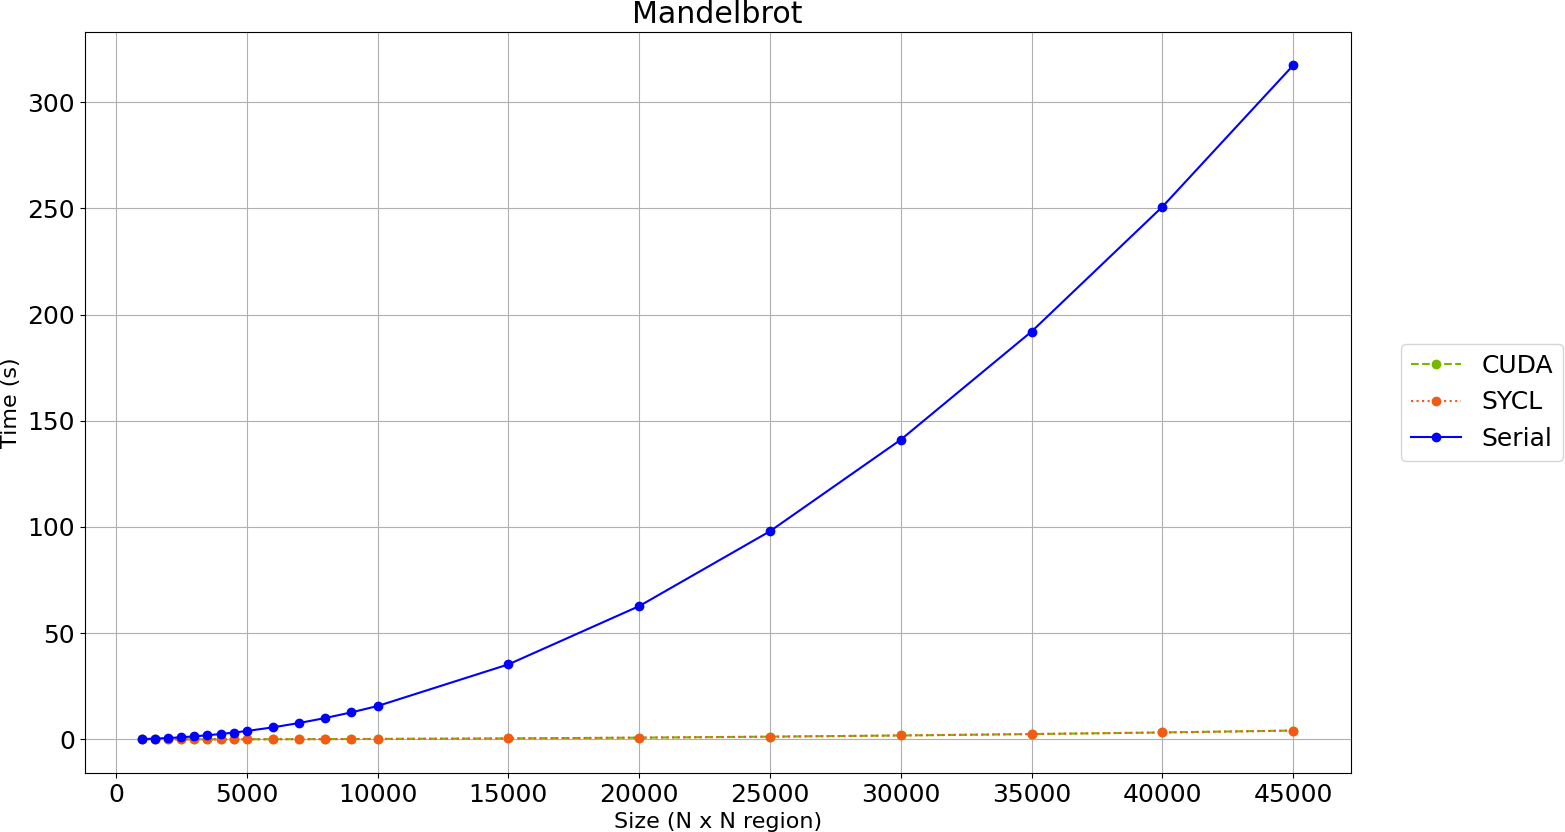
\includegraphics[width=\textwidth]{Images/mandelbrot-sycl-cuda-serial.png}
  \end{center}
\end{frame}
% -------------------------------------------------------------------------
\begin{frame}{Benchmark Comparisons: Mandelbrot set}
  \begin{center}
  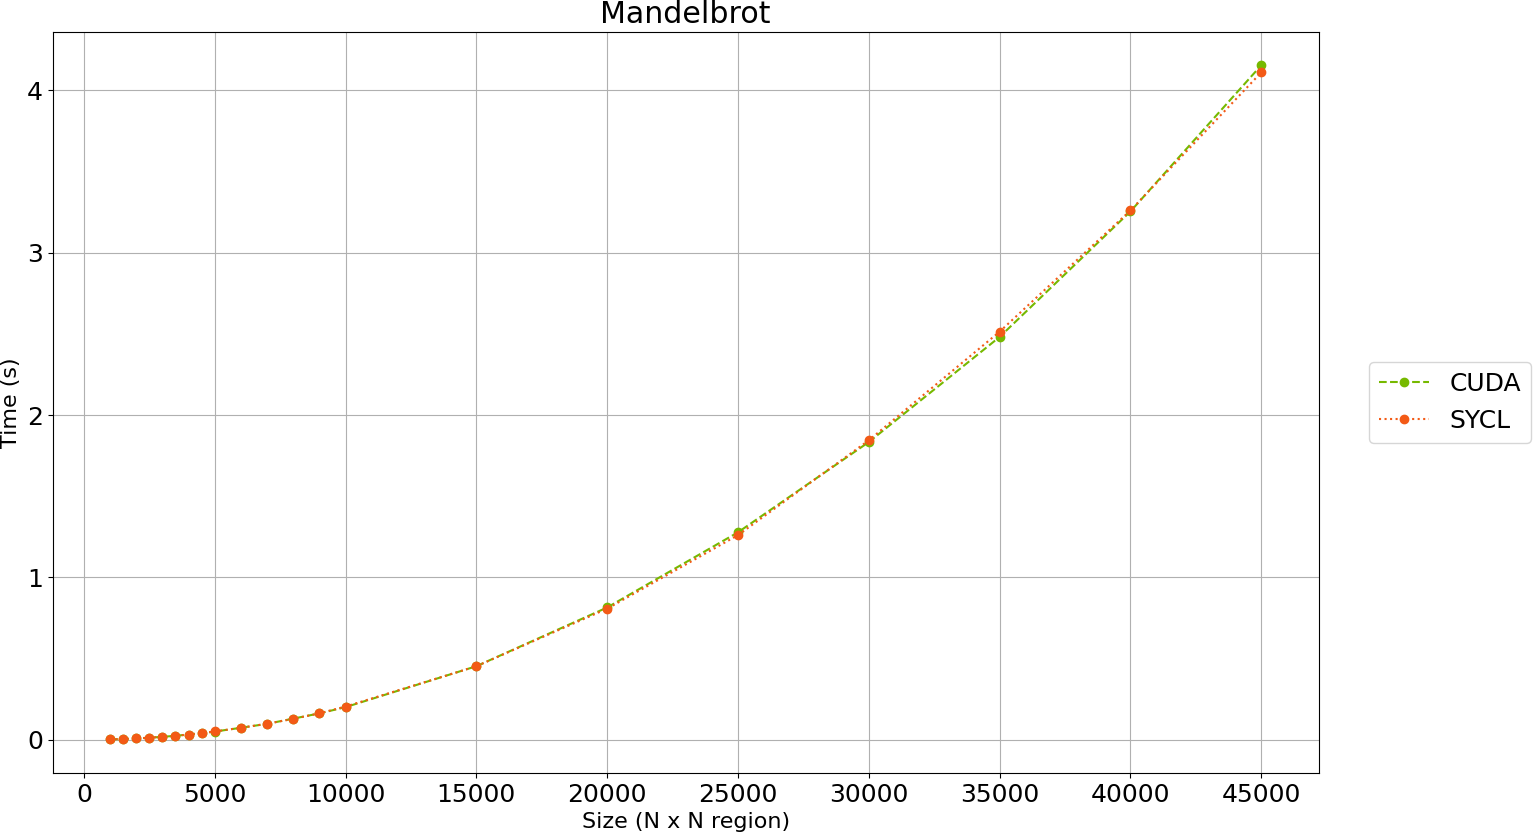
\includegraphics[width=\textwidth]{Images/mandelbrot-sycl-cuda.png}
  \end{center}
\end{frame}
% -------------------------------------------------------------------------
\begin{frame}{Benchmark Comparisons: Mandelbrot set}
  \begin{center}
  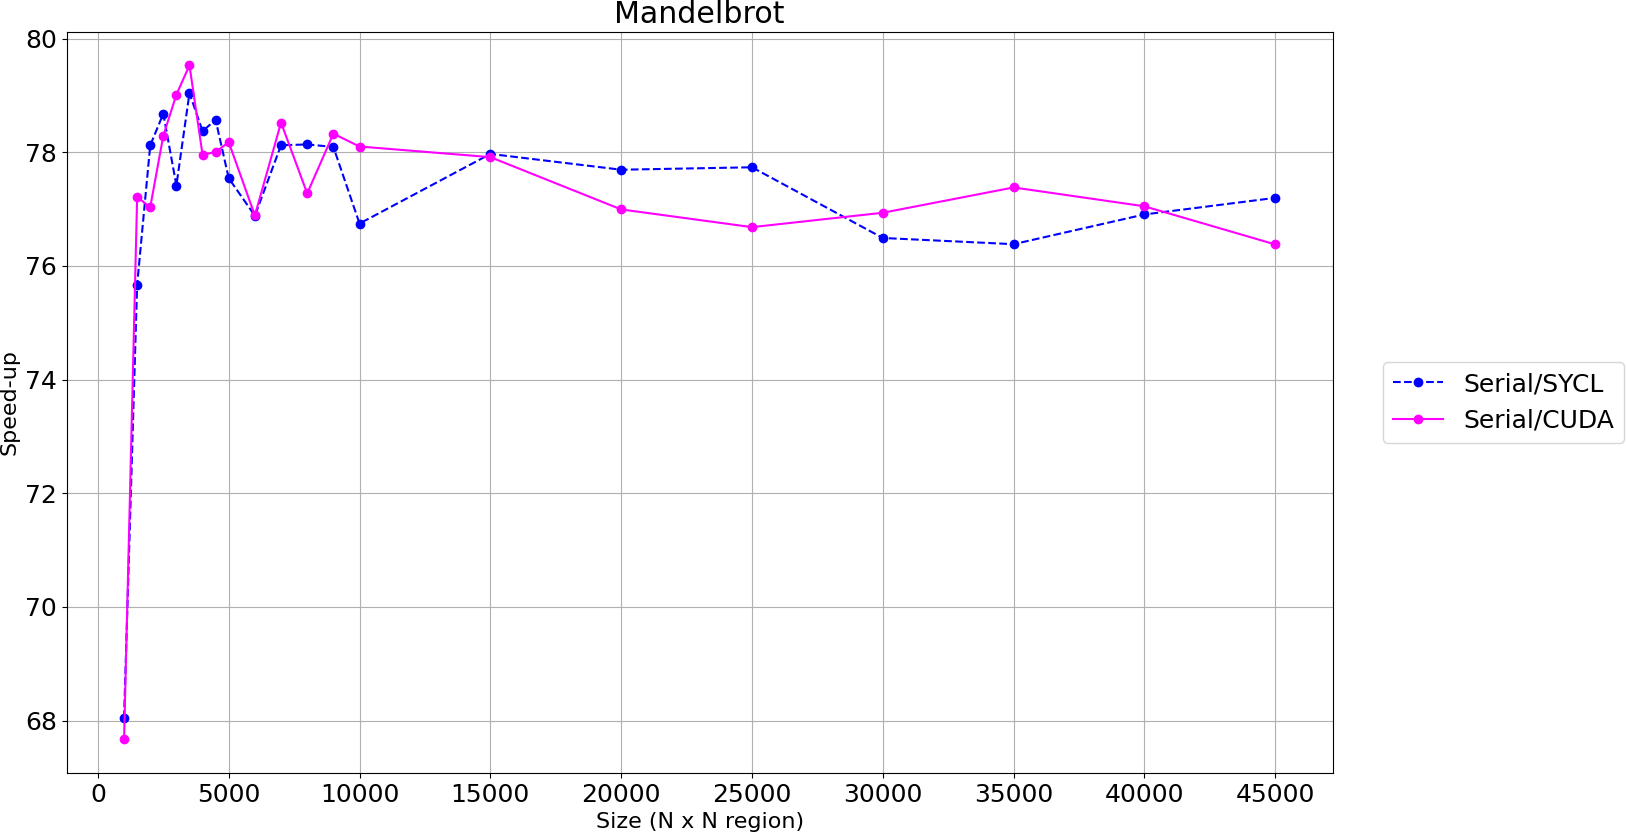
\includegraphics[width=\textwidth]{Images/mandelbrot-speed-up-sycl-cuda.png}
  \end{center}
\end{frame}
% -------------------------------------------------------------------------
\begin{frame}{Benchmark Comparisons: Floyd-Warshall algorithm}
  \begin{center}
  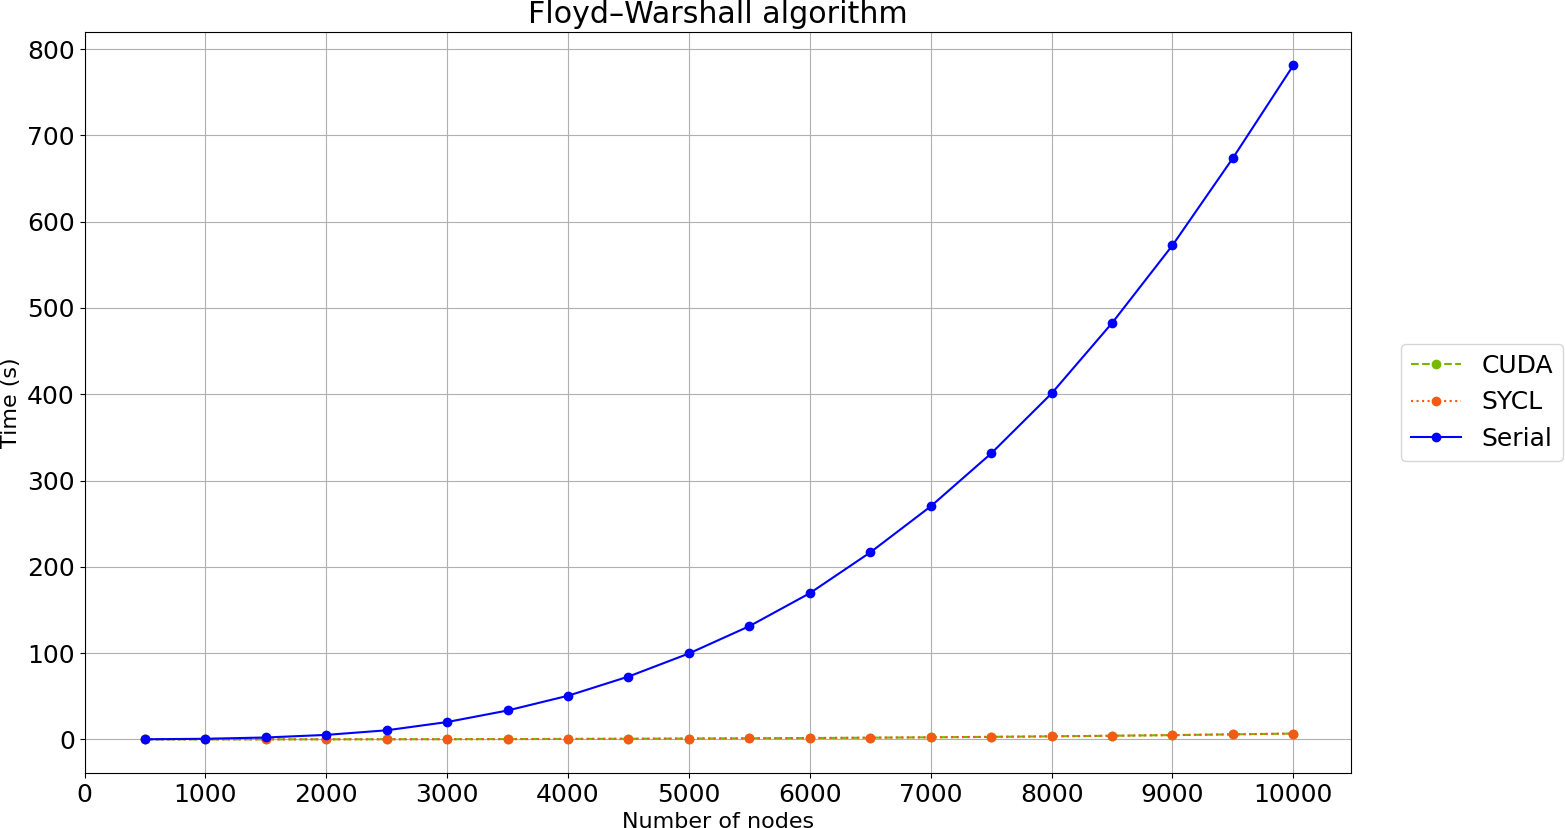
\includegraphics[width=\textwidth]{Images/floydwarshall-sycl-cuda-serial.png}
  \end{center}
\end{frame}
% -------------------------------------------------------------------------
\begin{frame}{Benchmark Comparisons: Floyd-Warshall algorithm}
  \begin{center}
  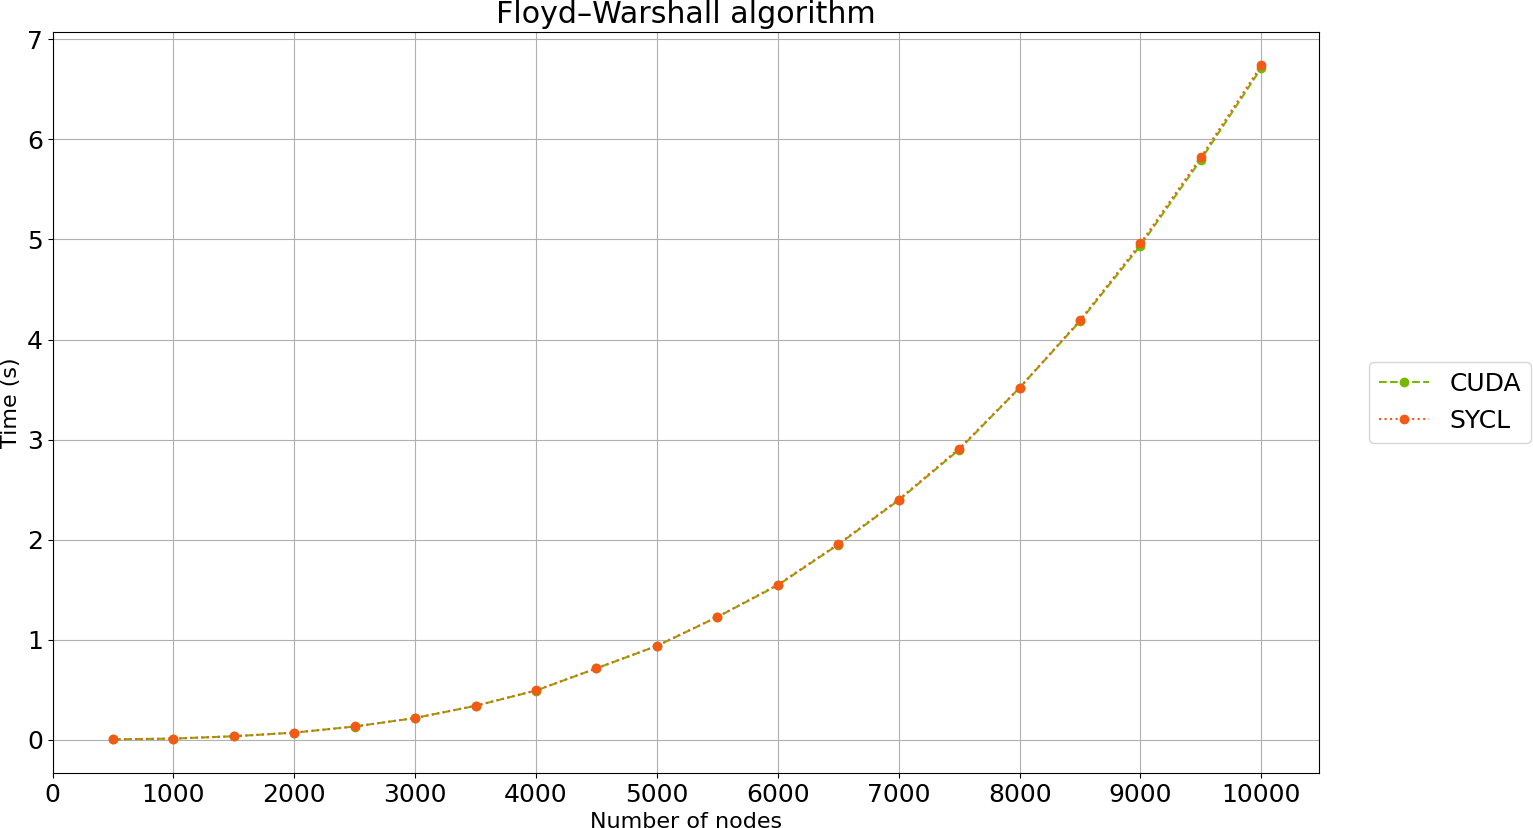
\includegraphics[width=\textwidth]{Images/floydwarshall-sycl-cuda.png}
  \end{center}
\end{frame}
% -------------------------------------------------------------------------
\begin{frame}{Benchmark Comparisons: Floyd-Warshall algorithm}
  \begin{center}
  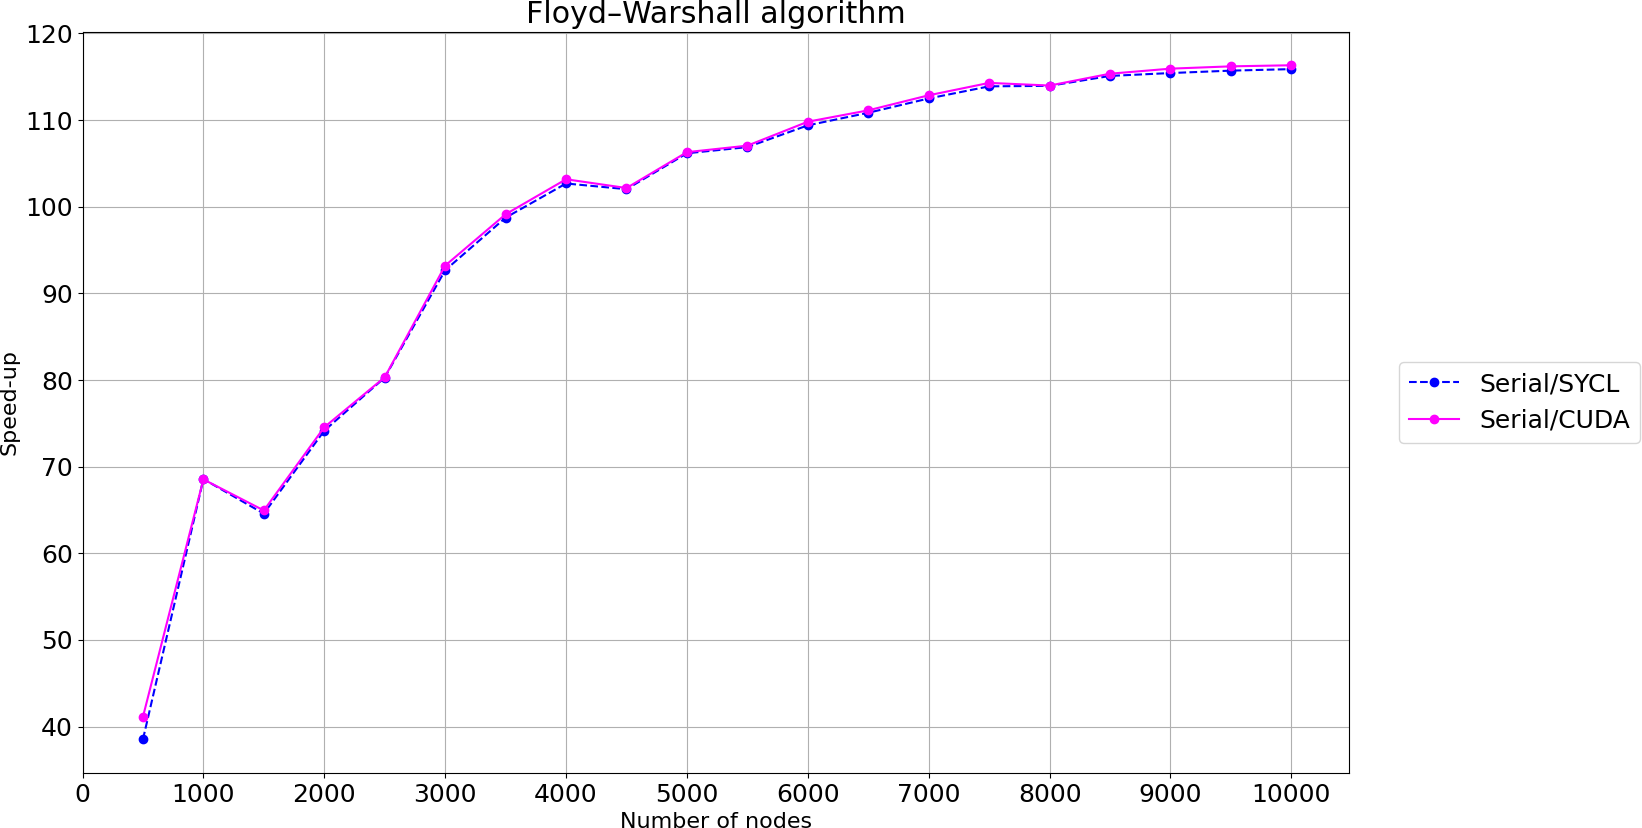
\includegraphics[width=\textwidth]{Images/floydwarshall-speed-up-sycl-cuda.png}
  \end{center}
\end{frame}
% -------------------------------------------------------------------------
\begin{frame}{Benchmark Comparisons: Molecular dynamics}
  \begin{center}
    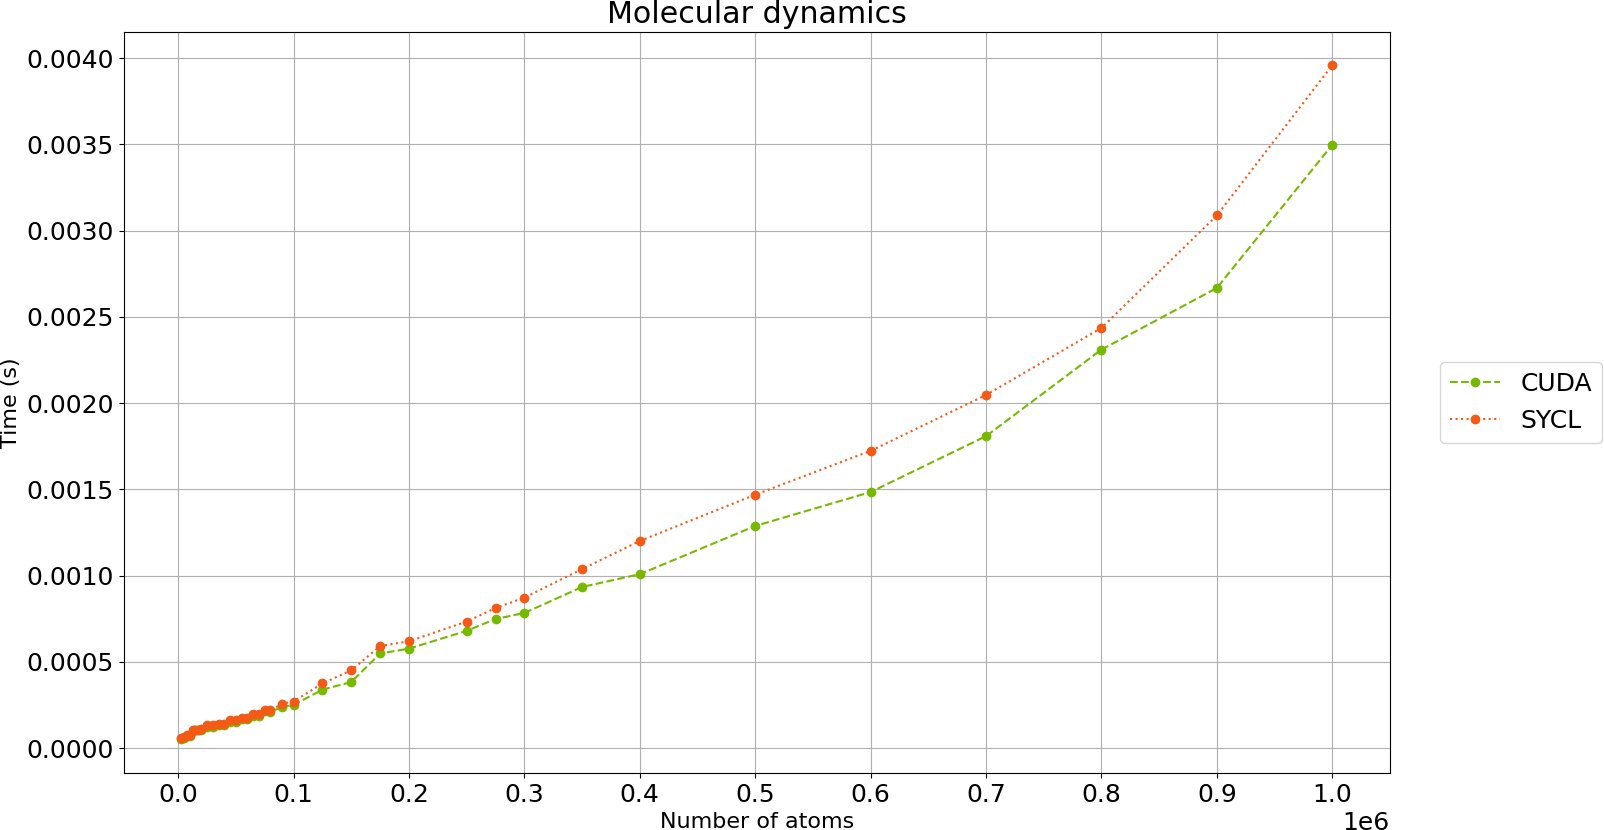
\includegraphics[width=\textwidth]{Images/md-sycl-cuda.png}
  \end{center}
\end{frame}
% -------------------------------------------------------------------------
\begin{frame}{Benchmark Comparisons: Molecular dynamics}
  Profiling GPU code with \textbf{NVIDIA Nsight Systems}
  \begin{center}
  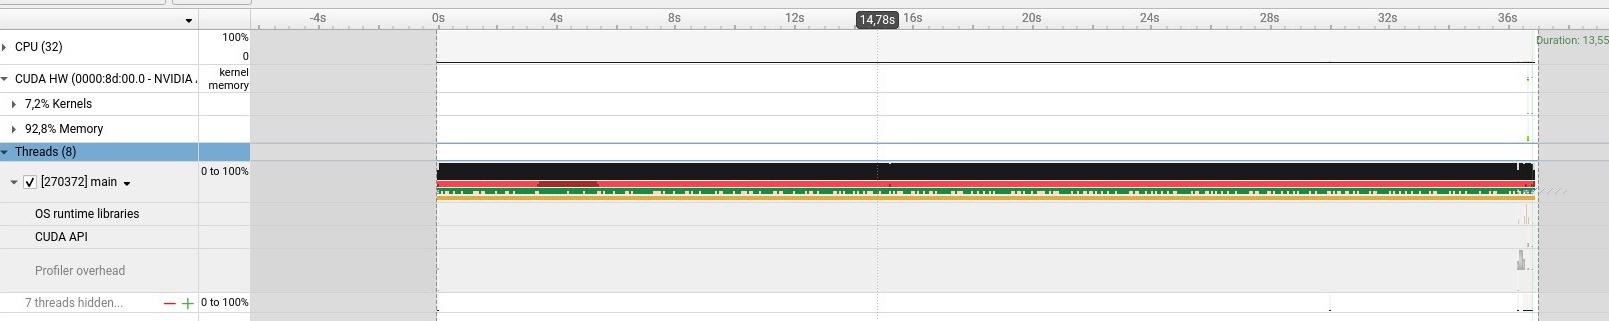
\includegraphics[width=\textwidth]{Images/nsight-all.jpeg}
  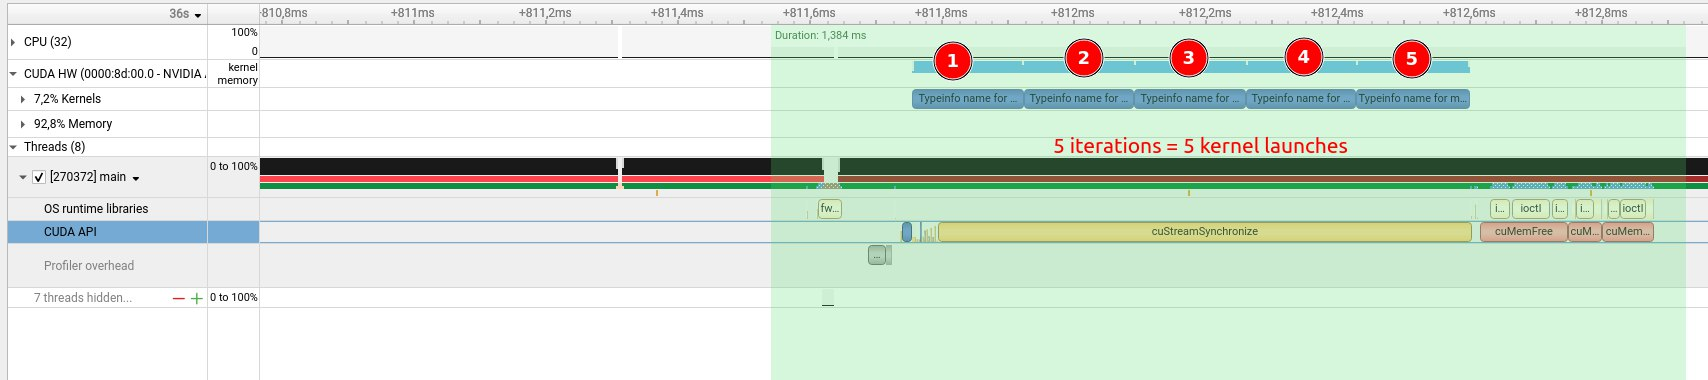
\includegraphics[width=\textwidth]{Images/nsight-kernel.jpeg}
  \end{center}
  \begin{columns}
    \begin{column}{0.48\textwidth}
      Total time: $\sim$37 seconds

      Total kernel time: $\sim$0.008 seconds
    \end{column}
  \end{columns}
\end{frame}
% -------------------------------------------------------------------------
\begin{frame}{Benchmark Comparisons: Backpropagation}
  \begin{center}
  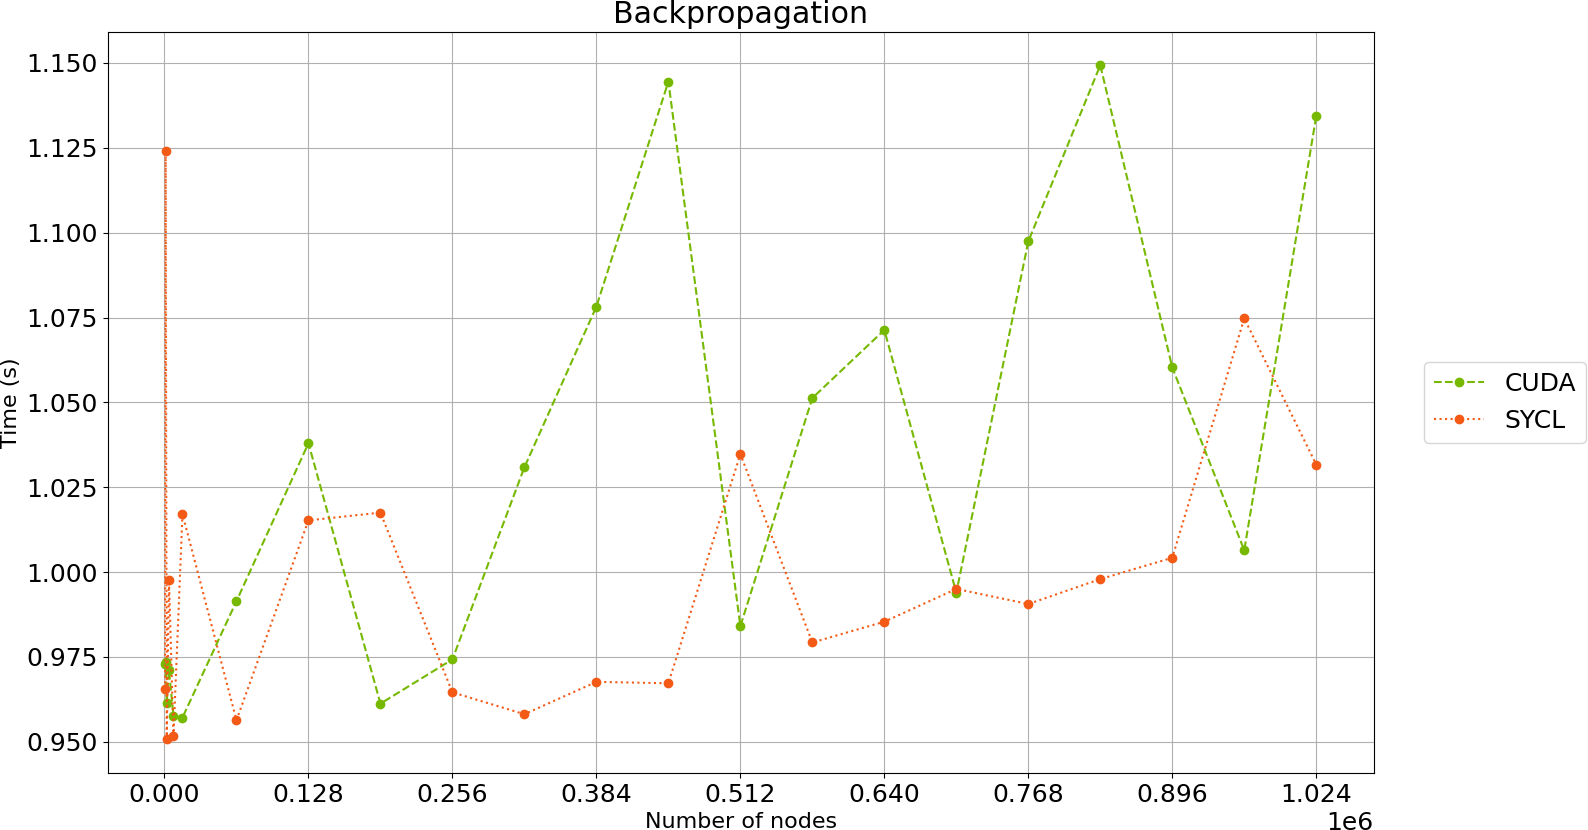
\includegraphics[width=\textwidth]{Images/backprop-sycl-cuda.png}
  \end{center}
\end{frame}
% -------------------------------------------------------------------------

\begin{frame}{Benchmark Comparisons: Backpropagation}
\centering
\lstinputlisting[language=C++,style=cppstyle]{Code/error_backprop_sycl.txt}
NDRange error on backpropagation benchmark
\end{frame}
